\begin{frame}{Shrinkage Methods}{Another Formulation for Ridge Regression and the Lasso}

The ridge and lasso regression coefficient estimates solve the problems: \pause

        \begin{equation}\label{eq:min-ridge}
        \underset{\beta}{\text{minimize}} \left\{     \sum_{i=1}^n \left(y_i - \beta_0 - \sum_{j=1}^p  \beta_j x_{ij} \right)^2  \right\} \text{ subject to }   \sum_{j=1}^p \beta_j^2 \leq s
    \end{equation} \pause 

    \begin{equation}\label{eq:min-lasso}
        \underset{\beta}{\text{minimize}} \left\{     \sum_{i=1}^n \left(y_i - \beta_0 - \sum_{j=1}^p  \beta_j x_{ij} \right)^2  \right\} \text{ subject to }  \sum_{j=1}^p |\beta_j| \leq s
    \end{equation} \pause \\

We find the coefficient that lead to the smallest RSS, subject to the constraint that there is a \textit{budget} $s$ forr how large the penalty can be. \pause 

    $\rightarrow$ $\forall \, \lambda \, \exists \, s$, such that the equation (\ref{eq:min-ridge}) will give the ridge estimates. \pause \\ 
    $\rightarrow$ $\forall \, \lambda \, \exists \, s$, such that the equation (\ref{eq:min-lasso}) will give the lasso estimates. 

\end{frame}

\begin{frame}{Shrinkage Methods}{Another Formulation for Ridge Regression and the Lasso}

\begin{itemize}
    \item When $p=2$, \pause 
        \begin{equation}
        \begin{aligned}
            \text{Rigde: } &\beta_1^2 + \beta_2^2 \leq s \qquad\qquad&
            \text{Lasso: } &|\beta_1 | + |\beta_2 | \leq s
        \end{aligned}    
        \end{equation} \pause 
    \item Let the OLS solution be $\hat{\beta}$. \pause 
    \item Let's represent the contours of $\hat{\beta}$ as ellipses centered around $\hat{\beta}$. \pause
    
    \begin{figure}
        \centering
        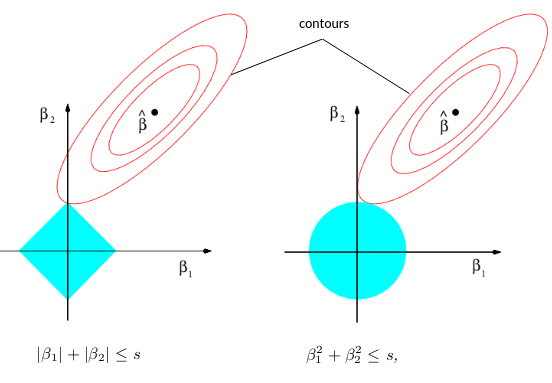
\includegraphics[height=4.5cm]{shrinkage/ridge-lasso.png}
    \end{figure} 
    
%    \item Coefficient are given by the first point at which an ellipse contacts the constraint region. 

%    \item Ridge regression has a circular constraint with no sharp points, this intersection will not generally occur on an axis, and so the ridge regression coefficient estimates will be exclusively non-zero. 

%    \item Lasso constraint has corners at each of the axes, and so the ellipse will often intersect the constraint region at an axis. When this occurs, one of the coefficients will equal zero.


\end{itemize}


\end{frame}
